% !TeX encoding = UTF-8

%% ------------------------------------------------------------------------
%% Copyright (C) 2021 SJTUG
%% 
%% SJTUBeamer Example Document by SJTUG
%% 
%% SJTUBeamer Example Document is licensed under a
%% Creative Commons Attribution-NonCommercial-ShareAlike 4.0 International License.
%% 
%% You should have received a copy of the license along with this
%% work. If not, see <http://creativecommons.org/licenses/by-nc-sa/4.0/>.
%% -----------------------------------------------------------------------

\documentclass[xcolor=table,dvipsnames,svgnames,aspectratio=169]{ctexbeamer}
% 可以通过 fontset=macnew / fontset=ubuntu / fontset=windows 选项切换字体集

\usepackage{tikz}
\usepackage[normalem]{ulem}
\usetikzlibrary{arrows}
\usepackage{amsmath}
\usepackage{mflogo}
\usepackage{graphicx}
\usepackage{xspace}
\usepackage{amsmath}
\usepackage{unicode-math}
\usepackage{ccicons}
\usepackage{hologo}
\usepackage{colortbl}
\usepackage{shapepar}
\usepackage{hyperxmp}
\usepackage{booktabs}
\usepackage{qrcode}
\usepackage{listings}
\usepackage{tipa}
\usepackage{multicol}
\usepackage{datetime2}
\usepackage{fontawesome5}
\usepackage{hyperref}
\usepackage[backend=biber,style=gb7714-2015]{biblatex}

\addbibresource{thesis.bib}
\setbeamertemplate{bibliography item}[text]

\graphicspath{{figures/}}

\hypersetup{
  pdfsubject = {上海交通大学图书馆专题培训讲座},
  pdfauthor = {Alexara Wu},
  pdfcopyright = {Licensed under CC-BY-SA 4.0. Some rights reserved.},
  pdflicenseurl = {http://creativecommons.org/licenses/by-sa/4.0/},
  unicode            = true,
  psdextra           = true,
  pdfdisplaydoctitle = true
}

\pdfstringdefDisableCommands{
  \let\\\relax
  \let\quad\relax
  \let\hspace\@gobble
}

\renewcommand{\TeX}{\hologo{TeX}}
\renewcommand{\LaTeX}{\hologo{LaTeX}}
\newcommand{\BibTeX}{\hologo{BibTeX}}
\newcommand{\XeTeX}{\hologo{XeTeX}}
\newcommand{\pdfTeX}{\hologo{pdfTeX}}
\newcommand{\LuaTeX}{\hologo{LuaTeX}}
\renewcommand{\CTeX}{C\TeX}
\newcommand{\MiKTeX}{\hologo{MiKTeX}}
\newcommand{\MacTeX}{Mac\hologo{TeX}}
\newcommand{\beamer}{\textsc{beamer}}
\newcommand{\XeLaTeX}{\hologo{Xe}\kern-.13em\LaTeX{}}
\newcommand{\pdfLaTeX}{pdf\LaTeX{}}
\newcommand{\LuaLaTeX}{Lua\LaTeX{}}

\def\TeXLive{\TeX{} Live\xspace}
\let\TL=\TeXLive
\newcommand{\SJTUThesis}{\textsc{SJTUThesis}\xspace}
\newcommand{\SJTUBeamer}{\textsc{SJTUBeamer}\xspace}
\newcommand{\SJTUThesisVersion}{1.0.0rc7}
\newcommand{\SJTUThesisDate}{2020/7/31}

\newcommand\link[1]{\href{#1}{\faLink}}
\newcommand\pkg[1]{\texttt{#1}}

\def\cmd#1{\texttt{\color{DarkBlue}\footnotesize $\backslash$#1}}
\def\env#1{\texttt{\color{DarkBlue}\footnotesize #1}}
\def\cmdxmp#1#2#3{\small{\texttt{\color{DarkBlue}$\backslash$#1}\{#2\}\hspace{1em}\\ $\Rightarrow$\hspace{1em} {#3}\par\vskip1em}}

\lstset{
  language=[LaTeX]TeX,
  basicstyle=\ttfamily\footnotesize,
  tabsize=2,
  keywordstyle=\bfseries\ttfamily\color{cprimary},
  commentstyle=\sl\ttfamily\color[RGB]{100,100,100},
  stringstyle=\ttfamily\color[RGB]{50,50,50},
  extendedchars=true,
  breaklines=true,
}

\lstdefinestyle{style@inline}{
  basicstyle   = \ttfamily,
  keepspaces   = true
}
\lstMakeShortInline[style=style@inline]|

\usetheme[maxplus]{sjtubeamer}
% 使用 maxplus/max/min 切换标题页样式
% 使用 red/blue 切换主色调
% 使用 light/dark 切换亮/暗色模式
% 使用外样式关键词以获得不同的边栏样式
%   miniframes infolines  sidebar* 
%   default    smoothbars split	 
%   shadow     tree       smoothtree
% *siderbar 推荐与 max 一起使用。

% \tikzexternalize[prefix=build/]
% 如果您需要缓存 tikz 图像,请取消注释上一行,并在编译选项中添加 -shell-escape。

\author{Alexara Wu}
\institute[SJTUG]{上海交通大学 Linux 用户组}
\date{\the\year 年 \the\month 月}
\subject{LaTeX, 论文排版, SJTUThesis}

\title[\SJTUBeamer 示例文档] % 页脚显示标题
{\textbf{如何使用 \LaTeX 排版论文}} % 首页标题

\subtitle{\SJTUBeamer 示例文档}

\begin{document}

% 使用节目录
\AtBeginSection[]{
  \begin{frame}
    % \tableofcontents[currentsection]           % 传统节目录             
    \sectionpage                   % 节页
  \end{frame}
}

% 使用小节目录
\AtBeginSubsection[]{                  % 在每小节开始
  \begin{frame}
    % \tableofcontents[currentsection,currentsubsection]             % 传统小节目录             
    \subsectionpage                % 小节页
  \end{frame}
}

\maketitle

\begin{frame}{目录}
  \tableofcontents
\end{frame}

% !TeX encoding = UTF-8
% !TeX root = ../main.tex

%% ------------------------------------------------------------------------
%% Copyright (C) 2021-2023 SJTUG
%% 
%% SJTUBeamer Example Document by SJTUG
%% 
%% SJTUBeamer Example Document is licensed under a
%% Creative Commons Attribution-NonCommercial-ShareAlike 4.0 International License.
%% 
%% You should have received a copy of the license along with this
%% work. If not, see <http://creativecommons.org/licenses/by-nc-sa/4.0/>.
%% -----------------------------------------------------------------------

\section{简介}

\subsection{\TeX{} 与 \LaTeX{}}

\begin{frame}[fragile]{\TeX{} 与 \LaTeX{}}
  \begin{columns}[T]
    \column{.8\textwidth}
    \begin{itemize}
      \item \TeX\ (\textipa{/'tEx/},
            \textipa{/'tEk/})
            \begin{itemize}
              \item 最初由 高德纳 (Donald E.~Knuth) 于 1978 年开发的排版系统
              \item 名称源自 technology 的希腊语词根 $\tau\varepsilon\chi$ \par
                    发音接近“泰赫”,而非“泰克斯”
              \item 最新版本为 \TeX\ 3.141592653(2021年1月)
                    \link{https://tex.stackexchange.com/questions/581118/whats-new-in-tex-version-3-141592653}
              \item 漂亮、美观、稳定、通用
              \item 尤其擅长数学公式排版
            \end{itemize}
      \item \LaTeX\ (\textipa{/'la:tEx/}, \textipa{/'leItEk/})
            \begin{itemize}
              \item Leslie Lamport 开发的一种 \TeX{} 格式
              \item 在 \TeX 的基础上提供宏包, 降低使用门槛
              \item 极其丰富的宏包,提供扩展功能
              \item 广泛用于学术界,期刊会议论文模板
              \item 大学学位论文模板,如 \SJTUThesis
            \end{itemize}
    \end{itemize}
    \column{.2\textwidth}
    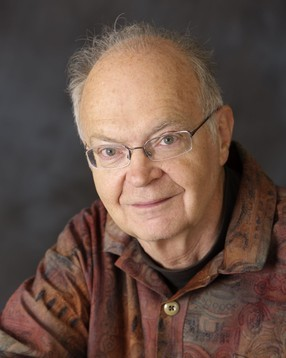
\includegraphics[height=.4\textheight]{Knuth.jpg}

    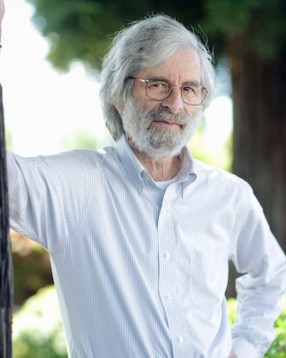
\includegraphics[height=.4\textheight]{Lamport.jpg}
  \end{columns}
\end{frame}

\begin{frame}{和 Word 对比}
  术业有专攻,评价需客观!
  \begin{table}[h]
    \centering
    \begin{tabular}{c|c}
      Microsoft\textsuperscript{\textregistered}  Word & \LaTeX
      \\
      \hline
      字处理工具                                            & 专业排版软件        \\
      容易上手,简单直观                                        & 容易上手          \\
      所见即所得                                            & 所见即所想,所想即所得   \\
      高级功能不易掌握                                         & 进阶难,但一般用不到    \\
      处理长文档需要丰富经验                                      & 和短文档处理基本无异    \\
      花费大量时间调格式                                        & 无需担心格式,专心作者内容 \\
      公式排版差强人意                                         & 尤其擅长公式排版      \\
      二进制格式,兼容性差                                       & 文本文件,易读、稳定    \\
      付费商业许可                                           & 自由免费使用        \\
    \end{tabular}
  \end{table}
\end{frame}

\begin{frame}{\TeX{}排版举例:公式}
  \begin{alertblock}{无编号公式}
    \begin{equation*}
      \mathcal{F}(\xi)=\int_{-\infty}^{\infty} f(x)\mathrm{e}^{-\mathrm{j}2\pi
      \xi x}\,\mathrm{d}x
    \end{equation*}
  \end{alertblock}
  \begin{alertblock}{多行多列公式}
    % Taken from Mathmode.tex
    \begin{align}
      y      & =d                  & z & =1                  \\
      y      & =cx+d               & z & =x+1                \\
      y_{12} & =bx^{2}+cx+d        & z & =x^{2}+x+1\nonumber \\
      y(x)   & =ax^{3}+bx^{2}+cx+d & z & =x^{3}+x^{2}+x+1
    \end{align}
  \end{alertblock}
\end{frame}

\begin{frame}{\TeX{}排版举例:公式}
  \begin{alertblock}{编号多行公式}
    % Taken from Mathmode.tex
    \begin{multline}
      A=\lim_{n\rightarrow\infty}\Delta x\left(a^{2}+\left(a^{2}+2a\Delta
      x+\left(\Delta x\right)^{2}\right)\right.\label{eq:reset}\\
      +\left(a^{2}+2\cdot2a\Delta x+2^{2}\left(\Delta x\right)^{2}\right)\\
      +\left(a^{2}+2\cdot3a\Delta x+3^{2}\left(\Delta x\right)^{2}\right)\\
      +\ldots\\
      \left.+\left(a^{2}+2\cdot(n-1)a\Delta x+(n-1)^{2}\left(\Delta
      x\right)^{2}\right)\right)\\
      =\frac{1}{3}\left(b^{3}-a^{3}\right)
    \end{multline}
  \end{alertblock}
\end{frame}

\begin{frame}{\TeX{}排版举例:图形}
  % https://texample.net/tikz/examples/3d-cone/
  \begin{tikzpicture}[join=round]
    \tikzstyle{conefill} = [fill=blue!20,fill opacity=0.8]
    \tikzstyle{ann} = [fill=white,font=\footnotesize,inner sep=1pt]
    \tikzstyle{ghostfill} = [fill=white]
    \tikzstyle{ghostdraw} = [draw=black!50]
    \filldraw[conefill](-.775,1.922)--(-1.162,.283)--(-.274,.5)
    --(-.183,2.067)--cycle;
    \filldraw[conefill](-.183,2.067)--(-.274,.5)--(.775,.424)
    --(.516,2.016)--cycle;
    \filldraw[conefill](.516,2.016)--(.775,.424)--(1.369,.1)
    --(.913,1.8)--cycle;
    \filldraw[conefill](-.913,1.667)--(-1.369,-.1)--(-1.162,.283)
    --(-.775,1.922)--cycle;
    \draw(1.461,.107)--(1.734,.127);
    \draw[arrows=<->](1.643,1.853)--(1.643,.12);
    \filldraw[conefill](.913,1.8)--(1.369,.1)--(1.162,-.283)
    --(.775,1.545)--cycle;
    \draw[arrows=->,line width=.4pt](.274,-.5)--(0,0)--(0,2.86);
    \draw[arrows=-,line width=.4pt](0,0)--(-1.369,-.1);
    \draw[arrows=->,line width=.4pt](-1.369,-.1)--(-2.1,-.153);
    \filldraw[conefill](-.516,1.45)--(-.775,-.424)--(-1.369,-.1)
    --(-.913,1.667)--cycle;
    \draw(-1.369,.073)--(-1.369,2.76);
    \draw(1.004,1.807)--(1.734,1.86);
    \filldraw[conefill](.775,1.545)--(1.162,-.283)--(.274,-.5)
    --(.183,1.4)--cycle;
    \draw[arrows=<->](0,2.34)--(-.913,2.273);
    \draw(-.913,1.84)--(-.913,2.447);
    \draw[arrows=<->](0,2.687)--(-1.369,2.587);
    \filldraw[conefill](.183,1.4)--(.274,-.5)--(-.775,-.424)
    --(-.516,1.45)--cycle;
    \draw[arrows=<-,line width=.4pt](.42,-.767)--(.274,-.5);
    \node[ann] at (-.456,2.307) {$r_0$};
    \node[ann] at (-.685,2.637) {$r_1$};
    \node[ann] at (1.643,.987) {$h$};
    \path (.42,-.767) node[below] {$x$}
    (0,2.86) node[above] {$y$}
    (-2.1,-.153) node[left] {$z$};
    % Second version of the cone
    \begin{scope}[xshift=3.5cm]
      \filldraw[ghostdraw,ghostfill](-.775,1.922)--(-1.162,.283)--(-.274,.5)
      --(-.183,2.067)--cycle;
      \filldraw[ghostdraw,ghostfill](-.183,2.067)--(-.274,.5)--(.775,.424)
      --(.516,2.016)--cycle;
      \filldraw[ghostdraw,ghostfill](.516,2.016)--(.775,.424)--(1.369,.1)
      --(.913,1.8)--cycle;
      \filldraw[ghostdraw,ghostfill](-.913,1.667)--(-1.369,-.1)--(-1.162,.283)
      --(-.775,1.922)--cycle;
      \filldraw[ghostdraw,ghostfill](.913,1.8)--(1.369,.1)--(1.162,-.283)
      --(.775,1.545)--cycle;
      \filldraw[ghostdraw,ghostfill](-.516,1.45)--(-.775,-.424)--(-1.369,-.1)
      --(-.913,1.667)--cycle;
      \filldraw[ghostdraw,ghostfill](.775,1.545)--(1.162,-.283)--(.274,-.5)
      --(.183,1.4)--cycle;
      \filldraw[fill=red,fill
        opacity=0.5](-.516,1.45)--(-.775,-.424)--(.274,-.5)
      --(.183,1.4)--cycle;
      \fill(-.775,-.424) circle (2pt);
      \fill(.274,-.5) circle (2pt);
      \fill(-.516,1.45) circle (2pt);
      \fill(.183,1.4) circle (2pt);
      \path[font=\footnotesize]
      (.913,1.8) node[right] {$i\hbox{$=$}0$}
      (1.369,.1) node[right] {$i\hbox{$=$}1$};
      \path[font=\footnotesize]
      (-.645,.513) node[left] {$j$}
      (.228,.45) node[right] {$j\hbox{$+$}1$};
      \draw (-.209,.482)+(-60:.25) [yscale=1.3,->] arc(-60:240:.25);
      \fill[black,font=\footnotesize]
      (-.516,1.45) node [above] {$P_{00}$}
      (-.775,-.424) node [below] {$P_{10}$}
      (.183,1.4) node [above] {$P_{01}$}
      (.274,-.5) node [below] {$P_{11}$};
    \end{scope}
  \end{tikzpicture}
  \hspace{1cm}
  % https://texample.net/tikz/examples/line-junctions/
  \tikzstyle{block} = [draw,fill=blue!20,minimum size=2em]
  \def\radius{.7mm}
  \tikzstyle{branch}=[fill,shape=circle,minimum size=3pt,inner sep=0pt]
  \begin{tikzpicture}[>=latex']
    \foreach \y in {1,2,3,4,5} {
        \node at (0,-\y) (input\y) {$i_\y$};
        \node[block] at (2,-\y) (block\y) {$f_\y$};
        \draw[->] (input\y) -- (block\y);
        \draw[->] (block\y.east) -- +(0.5,0);
      }
    \node[block] at (2,-6) (block6) {$f_6$};
    \draw[->] (block6.east) -- +(0.5,0);
    \path (input1) -- coordinate (branch) (block1);
    \tikzstyle{s}=[shift={(0mm,\radius)}]
    \draw[->] (branch) node[branch] {}{ % draw branch junction
      \foreach \c in {2,3,4,5} {
          [shift only] -- ([s]input\c -| branch) arc(90:-90:\radius)
        }
    } |- (block6);
  \end{tikzpicture}
\end{frame}

\begin{frame}{\TeX{}排版举例:文档}
  \begin{columns}
    \begin{column}{.45\textwidth}
      \begin{figure}[h]
        \centering
        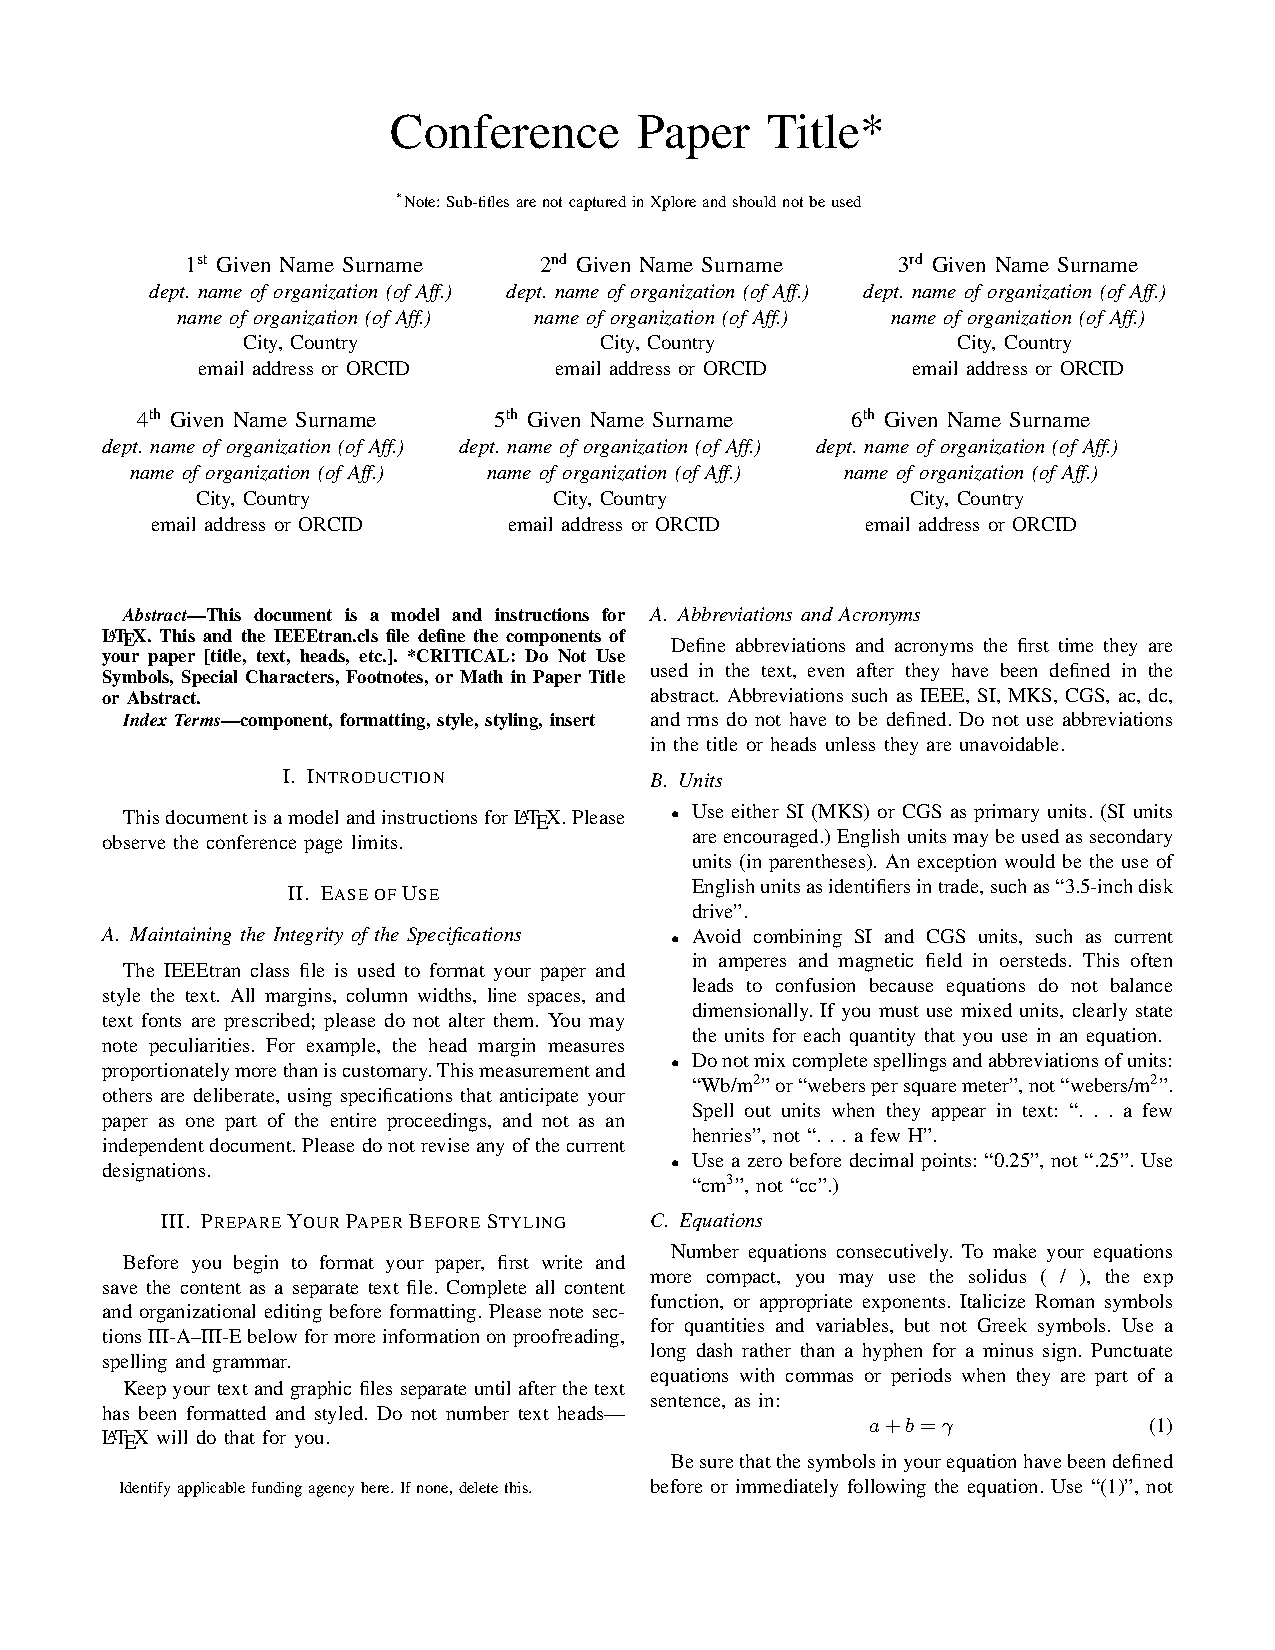
\includegraphics[width=.8\textwidth]{ieee-conference-template.pdf}
      \end{figure}
    \end{column}
    \begin{column}{.45\textwidth}
      \color{red}
      \heartpar{\footnotesize%
        Lorem ipsum dolor sit amet, consectetur adipisicing elit, sed do
        eiusmod
        tempor incididunt ut labore et	dolore magna aliqua. Ut enim ad minim
        veniam, quis nostrud exercitation ullamco laboris nisi ut aliquip ex ea
        commodo consequat. Duis aute irure dolor in reprehenderit in voluptate
        velit esse cillum dolore eu fugiat nulla pariatur. Excepteur sint
        occaecat cupidatat non proident, sunt in culpa qui officia deserunt
        mollit anim id est laborum.}
    \end{column}
  \end{columns}
\end{frame}

\begin{frame}{\TeX{}排版举例:幻灯片}
  \begin{columns}
    \begin{column}{.45\textwidth}
      \begin{figure}[h]
        \centering
        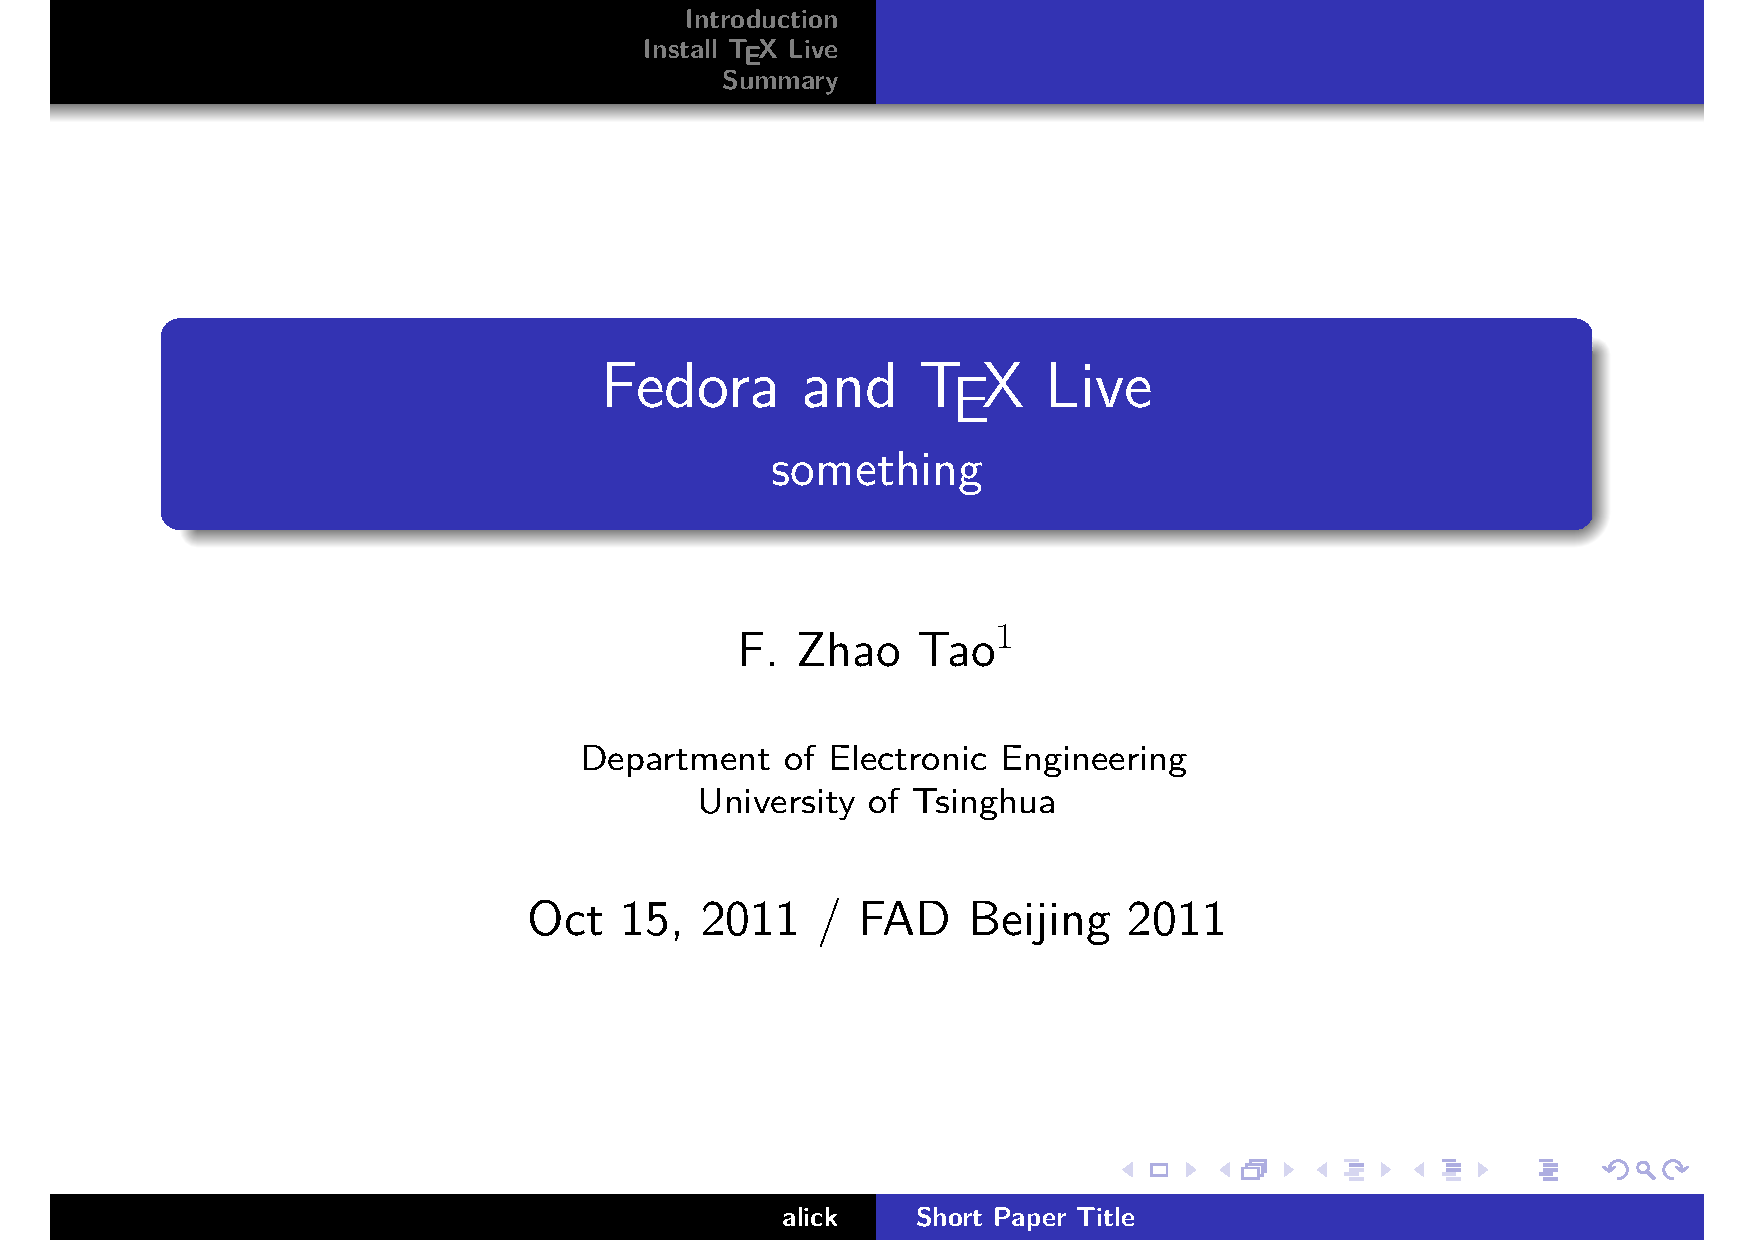
\includegraphics[width=\textwidth]{slides-beamer.pdf}
      \end{figure}
    \end{column}
    \begin{column}{.45\textwidth}
      \begin{figure}[h]
        \centering
        % https://www.overleaf.com/latex/templates/zut-fibeamer/ksnwzmnhktvn
        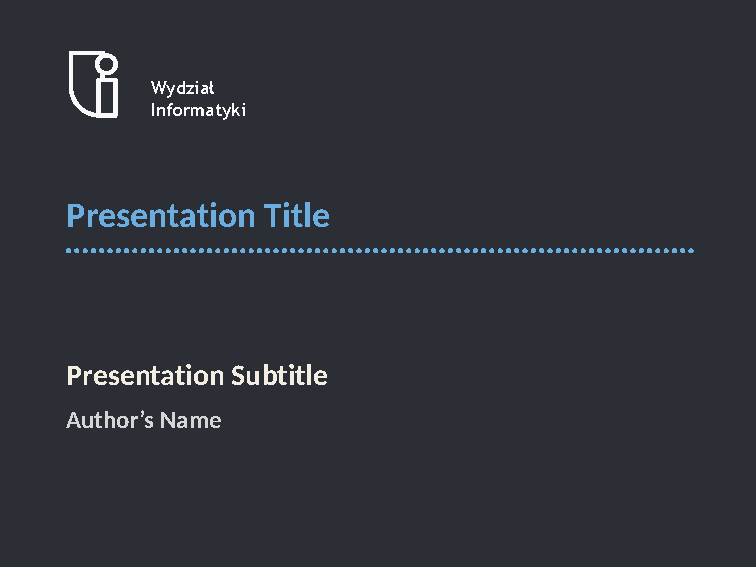
\includegraphics[width=\textwidth]{zut-fibeamer.pdf}
      \end{figure}
    \end{column}
  \end{columns}
\end{frame}

\subsection{安装}

\begin{frame}{如何安装 \hologo{(La)TeX}?}
  \begin{itemize}
    \item \TeX{}发行版(Distro)
          \begin{itemize}
            \item 引擎、宏包、字体、文档的综合体
            \item 常见\TeX{}发行版:
                  \alert{\TL}, \MacTeX, \MiKTeX, \CTeX
          \end{itemize}
    \item \TL
          \begin{itemize}
            \item 跨平台:Windows, Linux, macOS (\MacTeX{} $\approx$ \TL)
            \item 每年四月左右发布以年份命名的新版本,当前为 \TL{} 2023
            \item 官方维护,入门首选
          \end{itemize}
    \item \MiKTeX
          \begin{itemize}
            \item 最早专为 Windows 开发,现亦有 Linux 和 macOS 版本
            \item 宏包随用随装
            \item Christian Schenk 个人维护(是个狠人)
          \end{itemize}
    \item \CTeX
          \begin{itemize}
            \item 中科院吴凌云研究员基于 \MiKTeX 开发
            \item 极大的方便了中文 \TeX 用户
            \item 2012 年之后停止开发,\alert{不再建议}使用
          \end{itemize}
  \end{itemize}
\end{frame}

\begin{frame}[fragile]
  \frametitle{下载}
  \begin{itemize}
    \item 注意!
          \begin{itemize}
            \item 新手建议安装完整版 \TL{} (\MacTeX)
            \item 建议使用 ISO 镜像离线安装
            \item 在线安装要求网络稳定
            \item Windows 下不要放在带有中文的路径中
          \end{itemize}
    \item 选择国内 CTAN 镜像
          \begin{itemize}
            \item 上海交通大学 Linux 用户组 软件源镜像服务
                  \link{https://mirrors.sjtug.sjtu.edu.cn/}
            \item {\footnotesize
                  \url{https://mirrors.sjtug.sjtu.edu.cn/ctan/systems/texlive/Images/texlive.iso}
                  }
            \item 更多镜像 \link{http://mirror.ctan.org/README.mirrors}
          \end{itemize}
    \item 可选步骤:校验安装包
          \begin{itemize}
            \item \verb|Get-FileHash -Algorithm SHA512 texlive.iso|
            \item \verb|sha512sum --check texlive.iso.sha512|
          \end{itemize}
  \end{itemize}
\end{frame}

\begin{frame}[fragile]
  \frametitle{安装}
  \begin{itemize}
    \item Windows
          \begin{itemize}
            \item 挂载或解压下载的 ISO,运行 \verb|install-tl-windows.bat|
            \item 切换默认仓库为国内镜像(如 SJTUG)可加速今后升级
          \end{itemize}
    \item macOS
          \begin{itemize}
            \item 推荐使用独立的 pkg 安装包
                  \link{https://mirrors.sjtug.sjtu.edu.cn/ctan/systems/mac/mactex/MacTeX.pkg}
            \item 也可以使用 \TL 安装包安装
                  \link{http://www.tug.org/mactex/mactex-unix-download.html}
            \item 可选:Homebrew \link{https://brew.sh/}
          \end{itemize}
    \item Linux
          \begin{itemize}
            \item 不推荐从 Linux 发行版仓库直接安装(更新缓慢)
            \item 图形安装界面需要 Perl Tk 模块
                  \begin{lstlisting}[language=bash]
sudo apt-get install perl-tk
sudo ./install-tl -gui=perltk
        \end{lstlisting}
          \end{itemize}
  \end{itemize}
\end{frame}

\begin{frame}[fragile]
  \frametitle{安装(续)}
  \begin{itemize}
    \item Linux
          \begin{itemize}
            \item 添加环境变量到 \nolinkurl{~/.bashrc} 文件:
                  \begin{lstlisting}[language=sh]
export PATH=/usr/local/texlive/2023/bin/x86_64-linux:$PATH
export MANPATH=/usr/local/texlive/2023/texmf/doc/man:$MANPATH
export INFOPATH=/usr/local/texlive/2023/texmf/doc/info:$INFOPATH
          \end{lstlisting}
            \item 安装一个 dummy package,让系统的包管理器知道 \TL 已经装过了
                  \begin{itemize}
                    \item Debian/Ubuntu 用户参照手册做一个包即可
                          \link{https://www.tug.org/texlive/debian.html\#vanilla}
                    \item Arch Linux 用户装 AUR 里的 \verb|texlive-dummy|
                    \item Feodra 用户可以直接下载
                          \link{https://copr.fedoraproject.org/coprs/fatka/texlive-dummy/}
                  \end{itemize}
          \end{itemize}
    \item 安装指南
          \begin{itemize}
            \item 《一份简短的关于 \LaTeX{} 安装的介绍》
                  \link{https://mirrors.sjtug.sjtu.edu.cn/ctan/info/install-latex-guide-zh-cn/install-latex-guide-zh-cn.pdf}
            \item 《\TL{} 指南中文版》
                  \link{https://www.tug.org/texlive/doc/texlive-zh-cn/texlive-zh-cn.pdf}
            \item 更多参考:
                  \link{http://zhuanlan.zhihu.com/LaTeX/20069414}
                  \link{https://stone-zeng.github.io/2018-05-13-install-texlive-ubuntu/}
          \end{itemize}
  \end{itemize}
\end{frame}

\begin{frame}{选择编辑器}
  \begin{itemize}
    \item 专用编辑器
          \begin{itemize}
            \item TeXworks、TeXShop、\alert{TeXstudio}、TeXmaker、WinEdt 等
          \end{itemize}
    \item 通用编辑器(安装 \LaTeX{} 插件)
          \begin{itemize}
            \item Vim、Emacs、\alert{VS Code}、Sublime、Atom 等
          \end{itemize}
    \item 在线协作平台
          \begin{itemize}
            \item OverLeaf \link{https://www.overleaf.com/}, \TeX{} Page
                  \link{https://www.texpage.com}
            \item 交大 LaTeX 文档助手 \link{https://latex.sjtu.edu.cn/}(基于 OverLeaf)
          \end{itemize}
    \item 编辑器对比:\link{https://tex.stackexchange.com/q/339}
          \link{https://en.wikipedia.org/wiki/Comparison_of_TeX_editors}
          \link{https://www.zhihu.com/question/19954023}
  \end{itemize}
\end{frame}

\begin{frame}[fragile]{安装或更新宏包}
  \begin{itemize}
    \item 有时需要自己安装宏包
          \begin{itemize}
            \item 发行版没有预装
            \item 宏包需要更新
          \end{itemize}
    \item \TL
          \begin{itemize}
            \item 设置仓库地址 \verb|tlmgr option repository| {\footnotesize\ttfamily
                  https://mirrors.sjtug.sjtu.edu.cn/CTAN/systems/texlive/tlnet}
            \item \verb|tlmgr install <pkgname>| 安装、 \verb|tlmgr update --self --all| 全部更新
            \item \faWindows{} 开始菜单里找 TeX Live Manager
          \end{itemize}
    \item \MiKTeX
          \begin{itemize}
            \item \faWindows{} 开始菜单里找 MiKTeX Console
          \end{itemize}
  \end{itemize}
\end{frame}

% !TeX encoding = UTF-8
% !TeX root = ../main.tex

%% ------------------------------------------------------------------------
%% Copyright (C) 2021-2023 SJTUG
%% 
%% SJTUBeamer Example Document by SJTUG
%% 
%% SJTUBeamer Example Document is licensed under a
%% Creative Commons Attribution-NonCommercial-ShareAlike 4.0 International License.
%% 
%% You should have received a copy of the license along with this
%% work. If not, see <http://creativecommons.org/licenses/by-nc-sa/4.0/>.
%% -----------------------------------------------------------------------

\section{学术论文排版}
\subsection{\LaTeX{} 排版入门}

\begin{frame}[fragile]
  \frametitle{引擎与格式}
  \begin{itemize}
    \item \textbf{引擎}:\TeX{} 的实现

          \begin{itemize}
            \item \pdfTeX{}:直接生成 PDF,支持 micro-typography
            \item \XeTeX{}:支持 Unicode、OpenType 与复杂文字编排(CTL)
            \item \LuaTeX{}:支持 Unicode,内联 Lua,支持 OpenType
            \item (u)p\TeX{}:日本方面推动,生成 \verb|.dvi|,(支持 Unicode)
            \item Ap\TeX{}:底层 CJK 支持,内联 Ruby,Color Emoji
          \end{itemize}

    \item \textbf{格式}:\TeX{} 的语言扩展(命令封装)

          \begin{itemize}
            \item plain \TeX{}:Knuth 同志专用
            \item \LaTeX{}:排版科技类文章的事实标准
            \item Con\TeX t:基于 \LuaTeX{} 实现,优雅、易用(吗?)
          \end{itemize}

    \item \textbf{程序}:引擎 + dump 后的格式代码

          \begin{itemize}
            \item \alert{英文文章:\pdfLaTeX{}、\XeLaTeX{} 或 \LuaLaTeX{}}
            \item \alert{中文文章:\XeLaTeX{} 或 \LuaLaTeX{}}
          \end{itemize}
  \end{itemize}
\end{frame}

\begin{frame}[fragile]
  \frametitle{编译}
  \begin{itemize}
    \item 现代 \TeX{} 引擎均可直接生成 PDF
    \item 命令行

          \begin{itemize}
            \item \verb|pdflatex|/\verb|xelatex|/
                  \verb|lualatex| + \verb|<文件名>[.tex]|
            \item 多次编译:每次均需要读取并处理中间文件
            \item 推荐 \pkg{latexmk}\footnote{\MiKTeX 用户需要自行安装 perl 解释器}:运行
                  \verb|latexmk [<选项>] <文件名>| 即可自动完成所有工作
          \end{itemize}

    \item 编辑器

          \begin{itemize}
            \item 按钮的背后仍然是命令
            \item \verb|PATH| 环境变量:确定可执行文件的位置
            \item VS Code + \LaTeX{} Workshop:配置 \verb|tools| 和 \verb|recipes|
          \end{itemize}
  \end{itemize}
\end{frame}

\begin{frame}[fragile]{文件结构}
  \lstset{language=[LaTeX]TeX}
  \begin{lstlisting}[basicstyle=\ttfamily]
\documentclass[a4paper]{ctexart}
% 文档类型,如 ctexart,[]内是选项,如 a4paper
% 这里开始是导言区
\usepackage{graphicx} % 引用宏包
\graphicspath{{fig/}} % 设置图片目录
% 导言区到此为止
\begin{document}
这里开始是正文
\end{document}
  \end{lstlisting}
\end{frame}

\begin{frame}[fragile]{\LaTeX{}“命令”}
  \framesubtitle{宏 (Macro)、或者控制序列 (control sequence)}
  \begin{itemize}
    \item 简单命令
          \begin{itemize}
            \item \verb|\命令|\hspace{2em}
                  \verb|{\songti 中国人民解放军}| ~$\Rightarrow$ {\songti 中国人民解放军}
            \item \verb|\命令[可选参数]{必选参数}|\\
                  \verb|\section[精简标题]{这个题目实在太长了放到目录里面不太好看}|\\
                  $\Rightarrow$ {\heiti 1.1 \hspace{1em} \songti
                      这个题目实在太长了放到目录里面不太好看}
          \end{itemize}
    \item 环境
          \begin{columns}[c]
            \begin{column}{0.45\textwidth}
              \begin{lstlisting}[basicstyle=\ttfamily]
\begin{equation*}
  a^2-b^2=(a+b)(a-b)
\end{equation*}
              \end{lstlisting}
            \end{column}\hspace{1em}
            \begin{column}{0.45\textwidth}
              $ a^2-b^2=(a+b)(a-b)$
            \end{column}
          \end{columns}
  \end{itemize}
\end{frame}

\begin{frame}[fragile]{\LaTeX{} 常用命令}
  \begin{block}{简单命令}
    \centering
    \footnotesize
    \begin{tabular}{llll}
      \cmd{chapter}   & \cmd{section} & \cmd{subsection} & \cmd{paragraph}
      \\
      章               & 节             & 小节               & 带题头段落
      \\\hline
      \cmd{centering} & \cmd{emph}    & \cmd{verb}       & \cmd{url}
      \\
      居中对齐            & 强调            & 原样输出             & 超链接             \\\hline
      \cmd{footnote}  & \cmd{item}    & \cmd{caption}    &
      \cmd{includegraphics}                                                \\
      脚注              & 列表条目          & 标题               & 插入图片            \\\hline
      \cmd{label}     & \cmd{cite}    & \cmd{ref}
      \\
      标号              & 引用参考文献        & 引用图表公式等                            \\\hline
    \end{tabular}
  \end{block}
\end{frame}
\begin{frame}[fragile]{\LaTeX{} 常用环境}
  \begin{block}{环境}
    \centering
    \footnotesize
    \begin{tabular}{lll}
      \env{table}   & \env{figure}    & \env{equation}    \\
      表格            & 图片              & 公式                \\\hline
      \env{itemize} & \env{enumerate} & \env{description} \\
      无编号列表         & 编号列表            & 描述                \\\hline
    \end{tabular}
  \end{block}
\end{frame}
%
\begin{frame}{\LaTeX{}命令举例}
  \cmdxmp{chapter}{前言}{\heiti 第 1 章\hspace{1em} 前言}
  \cmdxmp{section[精简标题]}{这个题目实在太长了放到目录里面不太好看}{\heiti 1.1
    \hspace{1em} 这个题目实在太长了放到目录里面不太好看}
  \cmdxmp{footnote}{我是可爱的脚注}{前方高能\footnote{我是可爱的脚注}}
\end{frame}

\begin{frame}[fragile]{\LaTeX{} 环境举例}
  \begin{minipage}{0.4\linewidth}
    \begin{lstlisting}[basicstyle=\ttfamily\small]
\begin{itemize}
  \item 一条
  \item 次条
  \item 这一条可以分为 ...
    \begin{itemize}
      \item 子一条
    \end{itemize}
\end{itemize}
\end{lstlisting}
  \end{minipage}\hspace{1.5cm}
  \begin{minipage}{0.4\linewidth}
    \begin{itemize}
      \item 一条
      \item 次条
      \item 这一条可以分为 ...
            \begin{itemize}
              \item 子一条
            \end{itemize}
    \end{itemize}
  \end{minipage}
  \medskip

  \begin{minipage}{0.4\linewidth}
    \begin{lstlisting}
\begin{enumerate}
  \item 一条
  \item 次条
  \item 再条
\end{enumerate}
\end{lstlisting}
  \end{minipage}\hspace{1.5cm}
  \begin{minipage}{0.4\linewidth}
    \begin{enumerate}
      \item 一条
      \item 次条
      \item 再条
    \end{enumerate}
  \end{minipage}
\end{frame}
%

\begin{frame}[fragile]{\LaTeX{} 数学公式}

  \begin{columns}
    \begin{column}{.5\textwidth}
      \begin{lstlisting}[basicstyle=\ttfamily\small]
$V = \frac{4}{3}\pi r^3$

\[
  V = \frac{4}{3}\pi r^3
\]

\begin{equation}
\label{eq:vsphere}
V = \frac{4}{3}\pi r^3
\end{equation}
\end{lstlisting}
    \end{column}

    \begin{column}{.5\textwidth}
      $V = \frac{4}{3}\pi r^3$

      \[
        V = \frac{4}{3}\pi r^3
      \]

      \begin{equation}
        \label{eq:vsphere}
        V = \frac{4}{3}\pi r^3
      \end{equation}
    \end{column}
  \end{columns}

\end{frame}

\begin{frame}[fragile]{\LaTeX{} 数学公式}
  \begin{itemize}
    \item 数学公式排版是 \LaTeX{} 的绝对强项
    \item 数学排版需要进入数学模式,引用 \texttt{amsmath} 宏包
          \begin{itemize}
            \item 用单个美元符号(\verb|$|) 包围起来的内容是 {\bf 行内公式}
            \item 用两个美元符号(\verb|$$|) (不推荐)或
                  \verb|\[ \]| 包围起来的是 {\bf 单行公式} 或 {\bf 行间公式}
            \item 使用数学环境,例如 \texttt{equation} 环境内的公式会自动加上编号,
                  \texttt{align} 环境用于多行公式(例如方程组、多个并列条件等)
          \end{itemize}
    \item 寻找符号
          \begin{itemize}
            \item 运行 \texttt{texdoc symbols} 查看符号表
            \item S. Pakin. \emph{The Comprehensive \LaTeX{} Symbol List}
                  \link{https://ctan.org/pkg/comprehensive}
            \item 手写识别(有趣但不全):Detexify \link{http://detexify.kirelabs.org}
          \end{itemize}
    \item MathType 也可以使用和导出 \LaTeX{} 公式(不推荐)
  \end{itemize}
\end{frame}

%% 需要在导言区使用 \usepackage{unicode-math}
%
% \begin{frame}[fragile,label={frame:unicode-math}]{unicode-math:现代的数学输入方式}
%   \LaTeX{} 的公式确实很强大,但是……符号有点难记?

%   \pkg{unicode-math} 宏包提供了几乎所见即所得的公式输入:

%   \begin{itemize}
%     \item 可直接输入各类符号对应的 Unicode 字符(需要使用 UTF-8 编码):

%           \begin{columns}[c]
%             \begin{column}{0.45\textwidth}
%               \begin{lstlisting}
% \begin{equation*}
% ∫ Γ(x) dx = ±∞
% \end{equation*}
%       \end{lstlisting}
%             \end{column}\hspace{1em}
%             \begin{column}{0.45\textwidth}
%               \begin{equation*}
%                 ∫ Γ(x) dx = ±∞
%               \end{equation*}
%             \end{column}
%           \end{columns}
%     \item 使用 \verb|symbf| 等命令自动处理字母的粗体、斜体等变体,不必引入额外宏包。
%   \end{itemize}

%   \begin{columns}[c]
%     \begin{column}{0.45\textwidth}
%       \begin{lstlisting}
% \begin{align*}
% \symbf{\beta} &= \beta \symbf{I} \\
% \symbf{a} &= a \symbf{I}
% \end{align*}
% \end{lstlisting}
%     \end{column}\hspace{1em}
%     \begin{column}{0.45\textwidth}
%       \begin{align*}
%         \symbf{\beta} & = \beta \symbf{I} \\
%         \symbf{a}     & = a \symbf{I}
%       \end{align*}
%     \end{column}
%   \end{columns}

% \end{frame}

\begin{frame}[fragile]{层次与目录生成}
  \begin{columns}
    \begin{column}{.6\textwidth}

      \begin{lstlisting}[basicstyle=\ttfamily\small]
\tableofcontents % 这里是目录
\part{有监督学习}
\chapter{支持向量机}
\section{支持向量机简介}
\subsection{支持向量机的历史}
\subsubsection{支持向量机的诞生}
\paragraph{一些趣闻}
\subparagraph{第一个趣闻}
\end{lstlisting}
    \end{column}
    \begin{column}{.4\textwidth}
      第一部分\quad 有监督学习\\
      第一章\quad 支持向量机 \\
      1. 支持向量机简介 \\
      1.1 支持向量机的历史 \\
      1.1.1 支持向量机的诞生 \\
      一些趣闻  \\
      第一个趣闻
    \end{column}
  \end{columns}

\end{frame}

\begin{frame}[fragile]{列表与枚举}
  \begin{columns}
    \begin{column}{.6\textwidth}
      \begin{lstlisting}[basicstyle=\ttfamily\small]
\begin{enumerate}
\item \LaTeX{} 好处都有啥
  \begin{description}
    \item[好用] 体验好才是真的好
    \item[好看] 强迫症的福音
    \item[开源] 众人拾柴火焰高
  \end{description}
\item 还有呢?
  \begin{itemize}
    \item 好处 1
    \item 好处 2
  \end{itemize}
\end{enumerate}
\end{lstlisting}
    \end{column}
    \begin{column}{.4\textwidth}
      {\small
        \begin{enumerate}
          \item \LaTeX{} 好处都有啥
                \begin{description}
                  \item[好用] 体验好才是真的好
                  \item[好看] 治疗强迫症
                  \item[开源] 众人拾柴火焰高
                \end{description}
          \item 还有呢?
                \begin{itemize}
                  \item 好处 1
                  \item 好处 2
                \end{itemize}
        \end{enumerate}
      }
    \end{column}
  \end{columns}

\end{frame}

\begin{frame}[fragile]{交叉引用与插入插图}
  \begin{itemize}
    \item 给对象命名:图片、表格、公式等\\
          \verb|\label{name}|
    \item 引用对象\\
          \verb|\ref{name}|
  \end{itemize}
  \bigskip

  \begin{minipage}{0.7\linewidth}
    \begin{lstlisting}
交大校徽请参见图~\ref{fig:badge}。
\begin{figure}[htbp]
  \centering
  \includegraphics[height=.2\textheight]%
  {sjtu-badge-blue.pdf}
  \caption{交大校徽。}
  \label{fig:badge}
\end{figure}
\end{lstlisting}
  \end{minipage}\hfill
  \begin{minipage}{0.3\linewidth}\centering
    {\songti 交大校徽请参见图~1。}\\[1em]
    
\includegraphics[height=0.2\textheight]{sjtu-badge-blue.pdf}\\
    {\footnotesize\heiti 图~1. 交大校徽。}
  \end{minipage}
\end{frame}

\begin{frame}[fragile]{交叉引用与插入表格}
  \vspace{-1.5em}
  \begin{columns}
    \column{.6\textwidth}
    \begin{lstlisting}
\begin{table}[htbp]
   \caption{编号与含义}
   \label{tab:number}
   \centering
   \begin{tabular}{cl}
     \toprule
     编号 & 含义 \\
     \midrule
     1    & 第一 \\
     2    & 第二 \\
     \bottomrule
   \end{tabular}
\end{table}
公式~(\ref{eq:vsphere}) 中编号与含义
请参见表~\ref{tab:number}。
\end{lstlisting}
    \column{.4\textwidth}
    \centering
    {\small 表~1. 编号与含义}\\[2pt]
    \begin{tabular}{cl}\toprule
      编号 & 含义 \\\midrule
      1  & 第一 \\
      2  & 第二 \\\bottomrule
    \end{tabular}\\[5pt]

    \normalsize 公式~(\ref{eq:vsphere})编号与含义请参见表~1。
  \end{columns}
\end{frame}

\begin{frame}[fragile]{浮动体}
  \begin{itemize}
    \item 初学者最“捉摸不透”的特性之一
          \link{https://liam.page/2017/03/11/floats-in-LaTeX-basic}
    \item 图片和表格有时会很大,在插入的位置不一定放得下,因此需要浮动调整
    \item 避免在文中使用「下图」「上图」的说法,而是使用图表的编号,例如 \verb|图~\ref{fig:fig1}| 。
    \item \verb|\begin{figure}[<位置>] 图片 \end{figure}|
          \begin{itemize}
            \item 位置参数指定浮动体摆放的偏好
            \item \verb|h| 当前位置(here), \verb|t|
                  顶部(top), \verb|b| 底部(bottom),
                  \verb|p| 单独成页(p)
            \item \verb|!h| 表示忽略一些限制,\verb|H|
                  表示强制\alert{(强烈不建议,除非你知道自己在做什么)}
          \end{itemize}
    \item 温馨提示:图标题一般在下方,表标题一般在上方
  \end{itemize}
\end{frame}

\begin{frame}[fragile]
  \frametitle{作图与插图}
  \begin{itemize}
    \item 外部插入

          \begin{itemize}
            \item Mathematica、MATLAB
            \item PowerPoint、Visio、Adobe Illustrator、Inkscape
            \item Python \pkg{Matplotlib} 库、\texttt{Plots.jl}、R、Plotly 等
            \item draw.io \link{https://draw.io/}、ProcessOn \link{https://www.processon.com/}
                  等在线绘图网站
          \end{itemize}

    \item \TeX{} 内联

          \begin{itemize}
            \item Asymptote
            \item \alert{\pkg{pgf}/\pkg{TikZ}、\pkg{pgfplots}}
          \end{itemize}

    \item 插图格式

          \begin{itemize}
            \item 矢量图:\verb|.pdf|
            \item 位图:\verb|.jpg| 或 \verb|.png|
            \item \alert{不再推荐 \texttt{.eps}}
            \item 不(完全)支持 \verb|.svg|、\verb|.bmp|
          \end{itemize}

    \item 一些参考:\link{https://www.zhihu.com/question/21664179}
          \link{https://tex.stackexchange.com/q/158668}
          \link{https://tex.stackexchange.com/q/72930}
  \end{itemize}
\end{frame}

\begin{frame}[fragile]{表格绘制}
  \begin{itemize}
    \item 使用 \pkg{booktabs}、\pkg{longtables}、\pkg{multirow} 等宏包
    \item 手动绘制表格确实比较令人头疼,且较难维护
    \item 推荐使用在线工具绘制后导出代码:\LaTeX{} Table Generator
          \link{https://www.tablesgenerator.com/latex_tables}
  \end{itemize}
\end{frame}

\begin{frame}[fragile]{文献引用}
  \begin{itemize}
    \item 新时期我国信息技术产业的发展 \cite{devoftech}
    \item 他改变了中国 \cite{thelegendofjiang}
  \end{itemize}
\end{frame}

\begin{frame}[fragile]
  \frametitle{宏包推荐(先读文档后使用)}
  \vspace{-1.5em}
  \scriptsize
  \begin{multicols}{3}
    \begin{itemize}
      \item 必备

            \begin{itemize}
              \item \pkg{amsmath}
              \item \pkg{graphicx}
              \item \pkg{hyperref}
            \end{itemize}

      \item 样式

            \begin{itemize}
              \item \pkg{caption}
              \item \pkg{enumitem}
              \item \pkg{fancyhdr}
              \item \pkg{footmisc}
              \item \pkg{geometry}
              \item \pkg{titlesec}
            \end{itemize}

      \item 数学

            \begin{itemize}
              \item \pkg{bm}
              \item \pkg{mathtools}
              \item \pkg{physics}
              \item \pkg{unicode-math}
            \end{itemize}

      \item 表格

            \begin{itemize}
              \item \pkg{array}
              \item \pkg{booktabs}
              \item \pkg{longtable}
              \item \pkg{tabularx}
            \end{itemize}

      \item 插图、绘图

            \begin{itemize}
              \item \pkg{float}
              \item \pkg{pdfpages}
              \item \pkg{standalone}
              \item \pkg{subfigure}
              \item \pkg{pgf}/\pkg{tikz}
              \item \pkg{pgfplots}
            \end{itemize}

      \item 字体

            \begin{itemize}
              \item \pkg{newpx}
              \item \pkg{pifont}
              \item \pkg{fontspec}
            \end{itemize}

      \item 各种功能

            \begin{itemize}
              \item \pkg{algorithm2e}
              \item \pkg{beamer}
              \item \pkg{biblatex}
              \item \pkg{listings}
              \item \pkg{mhchem}
              \item \pkg{microtype}
              \item \pkg{minted}
              \item \pkg{natbib}
              \item \pkg{siunitx}
              \item \pkg{xcolor}
            \end{itemize}

      \item 多语言

            \begin{itemize}
              \item \pkg{babel}
              \item \pkg{polyglossia}
              \item \pkg{ctex}
              \item \pkg{xeCJK}
            \end{itemize}
    \end{itemize}
  \end{multicols}
  \vspace*{-0.5cm}
\end{frame}

\subsection{论文模板使用}

\begin{frame}{模板是什么?}
  \begin{itemize}
    \item 模板
          \begin{itemize}
            \item 已经设计好的格式框架
            \item 好的模板:使用户专注于内容
            \item 不应将时间花费在调整框架上
          \end{itemize}
    \item 再提 Office 和 Word
          \begin{itemize}
            \item 很少有人会有意识地在 Word 中使用模板
            \item 定义自己的标题?定义自己的列表?定义自己的段落样式?
            \item 自动化,还是手工调?
            \item 经常被折腾的精疲力竭
            \item 学习 \LaTeX{} 能帮助自己更好科学地使用 Word
          \end{itemize}
  \end{itemize}
\end{frame}

\begin{frame}{论文排版}
  \begin{itemize}
    \item 获取模板
          \begin{itemize}
            \item 随发行版自带、手动网络下载
            \item 模板文档类 \texttt{.cls} 文件
            \item 示例 \texttt{.tex} 文件
          \end{itemize}
    \item 编辑 \texttt{.tex} 文件:添加用户内容
    \item 编译:生成 PDF 文档
  \end{itemize}
\end{frame}

\begin{frame}[fragile]{论文排版举例}
  \begin{block}{IEEE 期刊论文}
    \begin{itemize}
      \item 获取模板:已随发行版自带
            \begin{itemize}
              \item 在安装目录 \verb|<prefix>/texlive/2023/texmf-dist/doc/latex/IEEEtran|
                    下找到 \verb|bare_jrnl.tex|
              \item 复制到某个文件夹(比如个人存论文的目录)
            \end{itemize}
      \item 编辑 \verb|bare_jrnl.tex| 文件 (英文模板:不支持中文)
      \item 编译
            \begin{itemize}
              \item 英文文献:\XeLaTeX{}、\pdfLaTeX{} 编译均可
            \end{itemize}
    \end{itemize}
  \end{block}
\end{frame}

% !TeX encoding = UTF-8
% !TeX root = ../main.tex

\section{学位论文排版}
\subsection{\SJTUThesis 上海交通大学学位论文模板}

\begin{frame}{\SJTUThesis}
  \framesubtitle{上海交通大学学位论文 \LaTeX{} 模板}
  \begin{itemize}
    \item 最早由韦建文于 2009 年 11 月发布 0.1a 版,2018 年起由 SJTUG 接手维护
    \item 最新版:\SJTUThesisVersion{} (\SJTUThesisDate)
    \item 支持本科、硕士、博士学位论文以及课程论文的排版
  \end{itemize}
  \begin{figure}[htbp]
    \centering
    
\includegraphics[height=.4\textheight]{sjtuthesis-bachelor-crop.pdf}\hspace{6pt}
    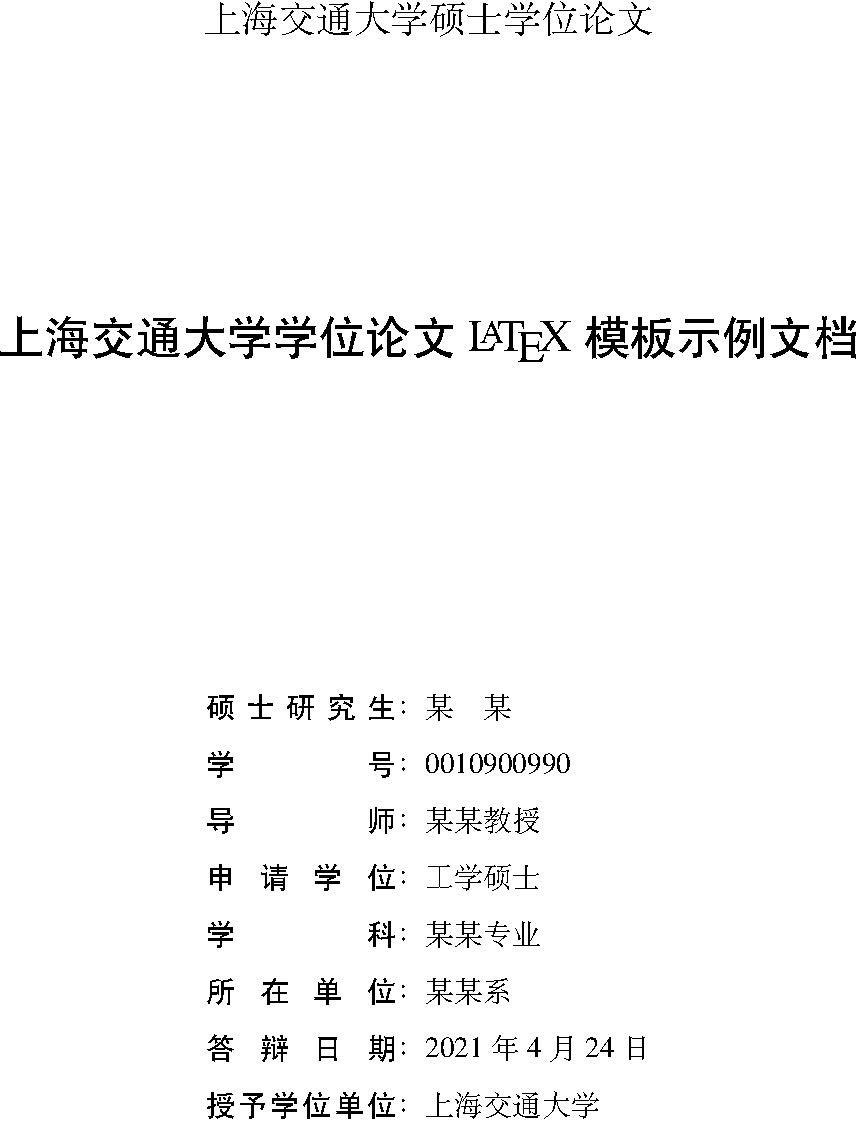
\includegraphics[height=.4\textheight]{sjtuthesis-master-crop.pdf}\hspace{6pt}
    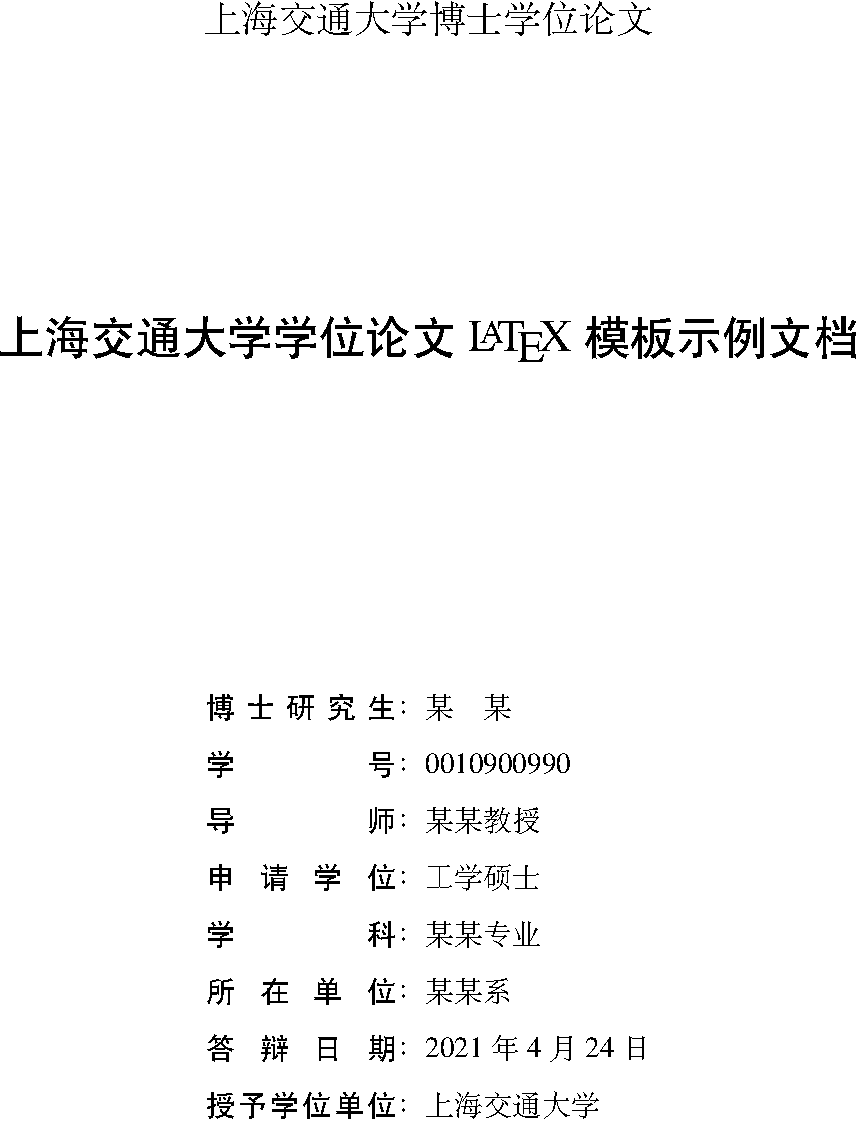
\includegraphics[height=.4\textheight]{sjtuthesis-doctor-crop.pdf}\hspace{6pt}
    
\includegraphics[height=.4\textheight]{sjtuthesis-course-crop.pdf}
  \end{figure}
\end{frame}

\begin{frame}[fragile]{获取\SJTUThesis{}}
  \begin{columns}
    \begin{column}{.65\textwidth}
      \begin{itemize}
        \item 下载最新版(推荐)
              \begin{itemize}
                \item GitHub Releases \link{https://github.com/sjtug/SJTUThesis/releases}
                \item OverLeaf \link{https://www.overleaf.com/latex/templates/sjtuthesis-latex-thesis-template-for-shanghai-jiao-tong-university/mkdwbyjbtfgg?r=b3b31f49&rm=d&rs=b}
              \end{itemize}
        \item 下载最新开发版(高级 / 想尝鲜 / 着急的用户)
              \begin{itemize}
                \item \url{https://github.com/sjtug/SJTUThesis}
                \item 切换到 |develop| 分支,点右边栏
                      \href{https://github.com/sjtug/SJTUThesis/archive/dev.zip}%
                      {Download ZIP} 按钮
              \end{itemize}
        \item 编译
              \begin{itemize}
                \item 解压缩看文档 |README.md|
                \item Windows: 双击 |Compile.bat| 脚本编译
                \item Linux \& macOS: 使用 |Makefile|
                \item 使用 |latexmk -xelatex main|
              \end{itemize}
      \end{itemize}
    \end{column}
    \begin{column}{.25\textwidth}
      \begin{figure}[htbp]
        \centering
        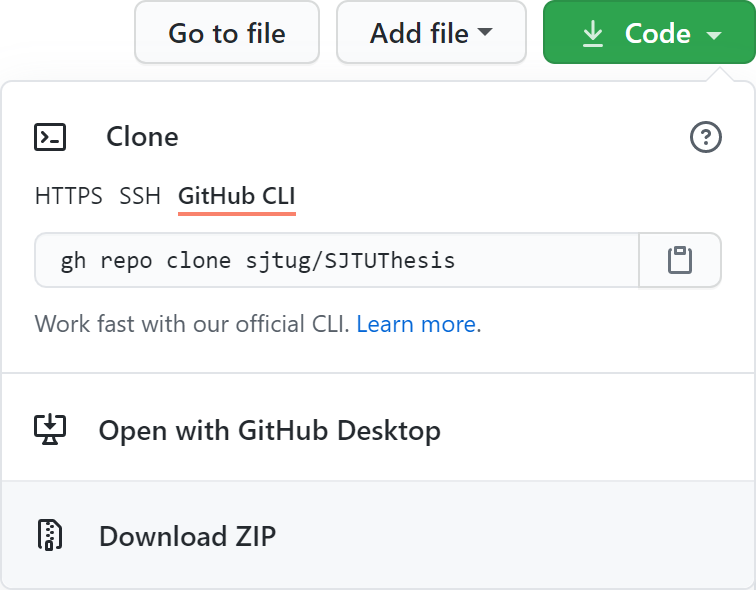
\includegraphics[width=\textwidth]{sjtuthesis-download.png}
      \end{figure}
      \vfill
    \end{column}
  \end{columns}
\end{frame}

\begin{frame}[fragile]{模板选项}
  \begin{description}
    \item[type] 指定论文类型(本科/硕士/博士/课程)
      \begin{lstlisting}[basicstyle=\ttfamily]
\documentclass[type=bachelor]{sjtuthesis}
  \end{lstlisting}
    \item[review] 开启盲审模式
      \begin{lstlisting}[basicstyle=\ttfamily]
\documentclass[type=master,review]{sjtuthesis}
  \end{lstlisting}
    \item[fontset] 指定字体(推荐使用 |windows|)
      \begin{lstlisting}[basicstyle=\ttfamily]
\documentclass[type=doctor,fontset=windows]{sjtuthesis}
  \end{lstlisting}
  \end{description}
\end{frame}

\begin{frame}[fragile]{模板设置}
  使用 |\sjtusetup| 命令指定论文各类设置:
  \begin{lstlisting}
\sjtusetup{
  info = {
    title             = {上海交通大学学位论文 \LaTeX{} 模板示例文档},
    title*            = {A Sample for \LaTeX-based SJTU Thesis Template},
    author            = {某\quad{}某},
    author*           = {Mo Mo},
  },
  style = {
    header-logo-color = red,
  },
  name = {
    publications      = {攻读学位期间完成的论文},
  },
}
  \end{lstlisting}
\end{frame}

\begin{frame}[fragile]{信息录入}
  |info| 域完成论文基本信息录入
  \begin{table}[h]
    \centering
    \footnotesize
    \begin{tabular}{lll} \toprule
      命令作用     & 中文对应选项                      & 英文对应选项      \\ \midrule
      论文标题     & |title|                           & |title*|          \\
      关键字列表   & |keywords|                        & |keywords*|       \\
      作者姓名     & |author|                          & |author*|         \\
      申请学位名称 & |degree|                          & |degree*|         \\
      院系名称     & |department|                      & |department*|     \\
      专业名称     & |major|                           & |major*|          \\
      导师         & |supervisor|                      & |supervisor*|     \\
      副导师       & |assisupervisor|                  & |assisupervisor*| \\
      日期         & \multicolumn{2}{c}{\texttt{date}}                     \\
      学号         & \multicolumn{2}{c}{\texttt{id}}                       \\ \bottomrule
    \end{tabular}
  \end{table}
\end{frame}

\begin{frame}[fragile]{数学}
  \begin{itemize}
    \item 公式示例:\nolinkurl{contents/math_and_citations.tex}
    \item \SJTUThesis{} 定义了常用的数学环境(需要手工引入 |amsthm| 宏包):
          \begin{table}[h]
            \centering
            \footnotesize
            \begin{tabular}{*{7}{l}}\toprule
              assumption & axiom   & conjecture & corollary   & definition & example  & exercise \\
              假设       & 公理    & 猜想       & 推论        & 定义       & 例       & 练习     \\\midrule
              lemma      & problem & proof      & proposition & remark     & solution & theorem  \\
              引理       & 问题    & 证明       & 命题        & 注         & 解       & 定理     \\\bottomrule
            \end{tabular}
          \end{table}
    \item \SJTUThesis{} 使用 \pkg{unicode-math} 进行数学输入(\ref{frame:unicode-math} 页),注意与传统方式的区别
  \end{itemize}
\end{frame}

\begin{frame}[fragile]{参考文献}
  \begin{itemize}
    \item 建议自动生成
          \begin{itemize}
            \item \LaTeX 引擎自身不能处理参考文献,需要借助外部程序!
          \end{itemize}
    \item 传统方法:\BibTeX 后端
          \begin{itemize}
            \item 控制文献、引用样式:\pkg{natbib} 宏包
            \item 国标样式:\pkg{gbt7714} 宏包 \link{https://mirrors.sjtug.sjtu.edu.cn/ctan/biblio/bibtex/contrib/gbt7714/gbt7714.pdf}
          \end{itemize}
    \item 现代方法:|biber| 后端 + \pkg{biblatex} 宏包
          \begin{itemize}
            \item 国标样式:\pkg{biblatex-gbt7714-2015} 宏包 \link{https://mirrors.sjtug.sjtu.edu.cn/ctan/macros/latex/contrib/biblatex-contrib/biblatex-gb7714-2015/biblatex-gb7714-2015.pdf}
          \end{itemize}
    \item 需要多轮编译——再次推荐 latexmk
  \end{itemize}
\end{frame}

\begin{frame}[fragile]{参考文献(续)}
  \begin{itemize}
    \item 生成 |.bib| 数据库
          \begin{itemize}
            \item Google Scholar 可直接复制或者批量导出
            \item 用 Zotero、Jabref 等文献管理软件生成
          \end{itemize}
    \item 两种引用模式:
          \begin{itemize}
            \item 上标模式:如“在许多文献\textsuperscript{[12-13]}中……”
                  \begin{lstlisting}[basicstyle=\ttfamily]
    \cite{key12, key13}
          \end{lstlisting}
            \item 正文模式:如“文献~[14] 证明了……”
                  \begin{lstlisting}[basicstyle=\ttfamily]
    \parencite{key14}
          \end{lstlisting}
          \end{itemize}
  \end{itemize}
\end{frame}

\begin{frame}[fragile]{\SJTUThesis 问题}
  \begin{itemize}
    \item 常见问题
          \begin{itemize}
            \item 参考文献列表出错、缺少字体、无法编译、格式不对……
            \item 阅读模板文档 |sjtuthesis.pdf| 和 SJTUThesis 示例文档代码
            \item 查看 FAQ \link{https://github.com/sjtug/SJTUThesis/wiki/常见问题}
          \end{itemize}
    \item 主动提问
          \begin{itemize}
            \item GitHub Issues 提问:\link{https://github.com/sjtug/SJTUThesis/issues}
          \end{itemize}
  \end{itemize}
\end{frame}

% !TeX encoding = UTF-8
% !TeX root = ../main.tex

%% ------------------------------------------------------------------------
%% Copyright (C) 2021-2023 SJTUG
%% 
%% SJTUBeamer Example Document by SJTUG
%% 
%% SJTUBeamer Example Document is licensed under a
%% Creative Commons Attribution-NonCommercial-ShareAlike 4.0 International License.
%% 
%% You should have received a copy of the license along with this
%% work. If not, see <http://creativecommons.org/licenses/by-nc-sa/4.0/>.
%% -----------------------------------------------------------------------

\section{总结}

\begin{frame}{常见 \LaTeX{} 困惑}
  \begin{itemize}
    \item \alert{编译不通过} 缺少必要宏包,命令拼写错误,括号未配对等
    \item \alert{表格图片乱跑} 非问题,\LaTeX{} 浮动定位算法
          \link{https://liam.page/2017/04/30/floats-in-LaTeX-the-positioning-algorithm/}
    \item \alert{段落间距变大} 非问题,\LaTeX{} 排版算法
    \item \alert{参考文献} 推荐使用 \BibTeX{} 或者 Bib\LaTeX{}(视模板而定),也可以手写 \cmd{bibitem}
          \link{https://github.com/hushidong/biblatex-gb7714-2015}
  \end{itemize}
\end{frame}

\begin{frame}{系统学习}
  \begin{itemize}
    \item 包太雷 《\LaTeX{} Notes(第二版)》~(3小时)(lnotes2)
          \link{http://dralpha.altervista.org/zh/tech/lnotes2.pdf}
    \item Stefan Kottwitz 《LaTeX Cookbook》
    \item WikiBooks:英文 \link{https://en.wikibooks.org/wiki/LaTeX}、中文
          \link{https://zh.wikibooks.org/wiki/LaTeX}
    \item 在线教程:OverLeaf 帮助文档 \link{https://www.overleaf.com/learn}
    \item 经典文档(亦可能比较过时)
          \begin{itemize}
            \item 仔细阅读《一份不太简短的~\LaTeXe{} 介绍》(lshort-zh-cn)~(1--2 天)
                  \link{https://mirrors.sjtug.sjtu.edu.cn/CTAN/info/lshort/chinese/lshort-zh-cn.pdf}
            \item 粗略阅读《\LaTeXe{} 插图指南》~(2--3 小时)
          \end{itemize}
    \item 从~\SJTUThesis{} 示例文档入手
  \end{itemize}
\end{frame}

\begin{frame}{扩展阅读}
  \begin{itemize}
    \item 一份其实很短的 \LaTeX 入门文档 (Liam Huang)
          \link{https://liam.page/2014/09/08/latex-introduction/}
    \item 网站推荐:
          \begin{itemize}
            \item http://www.latexstudio.net/
            \item http://www.chinatex.org/
          \end{itemize}
    \item 知乎 \LaTeX{} 专栏(偏技术)
          \link{http://zhuanlan.zhihu.com/LaTeX}
          % \item \LaTeX{}杂谈(刘海洋)
    \item 《\LaTeX{}入门》(刘海洋)
    \item 现代 LaTeX入门讲座(曾祥东)
          \link{https://github.com/stone-zeng/latex-talk/releases/tag/2019-04-18}
    \item “黑科技”:在 \LaTeX{} 中书写 Markdown 进行排版
          \link{https://liam.page/2020/03/30/writing-manuscript-in-Markdown-and-typesetting-with-LaTeX/}
  \end{itemize}
\end{frame}

\begin{frame}[fragile]{利用文档}
  \begin{itemize}
    \item 常用文档(\verb|texdoc <package>|)
          \begin{itemize}
            \item \pkg{symbols}: 符号大全
            \item \pkg{Mathmode}: 数学参考
            \item \pkg{ctex}, \pkg{xeCJK}: 中文支持
            \item \pkg{texlive-zh}: \TL 安装与使用
            \item 所用宏包文档
          \end{itemize}
    \item 工具
          \begin{itemize}
            \item \verb|tlmgr|: \TL 管理器
            \item \verb|texdoc|: \TeX{} 文档查看器\\
                  例如:\verb|texdoc lshort-zh-cn|
            \item 在线文档 \TeX{}doc \link{http://texdoc.net/}
            \item \TeX{}studio 和 WinEdt 都支持在帮助里看文档
          \end{itemize}
  \end{itemize}
\end{frame}

\begin{frame}{一点人生的经验}
  \begin{itemize}
    \item 不要着急安装,先在 OverLeaf 上熟悉各类操作
    \item 不要过于相信网上的中文文档
          \begin{itemize}
            \item 简单鉴别方法: 排版的好看程度
          \end{itemize}
    \item 湿兄用U盘拷给你的的 \CTeX{} 套装一定是过时的,\SJTUThesis{} 八成是老版本的
    \item 如果你要处理中文
          \begin{itemize}
            \item 使用 \XeLaTeX{}, 使用 \XeLaTeX{}, 使用 \XeLaTeX{}
            \item 忘记 \pkg{CJK}, 忘记 \pkg{CJK}, 忘记 \pkg{CJK}
            \item 使用 \pkg{ctex} 宏包(2.0以上版本)(跟 \CTeX{} 套装仅仅是名字像)
          \end{itemize}
    \item 写一点,编译一次,减小排错搜索空间
  \end{itemize}
\end{frame}

\begin{frame}[fragile]
  \frametitle{Git版本管理}
  \begin{itemize}
    \item 版本管理的必要性
          \begin{itemize}
            \item 远离「初稿,第二稿……终稿,终稿(打死也不改了)」命名
            \item 方便与他人协同合作
          \end{itemize}
    \item 基本用法
          \begin{itemize}
            \item 跟踪更改:\verb|git init|、\verb|git add|
                  \verb|git commit|
            \item 撤销与回滚:\verb|git reset|、\verb|git revert|
            \item 分支与高级用法:\verb|git branch|、\verb|git checkout|
                  \verb|git rebase|
            \item 远端仓库操作:\verb|git pull|、\verb|git push|、
                  \verb|git fetch|
            \item 推荐用 VS Code 等进行可视化操作
            \item 参考链接:\link{https://git-scm.com/book/en/v2}
                  \link{https://www.liaoxuefeng.com/wiki/0013739516305929606dd18361248578c67b8067c8c017b000}
          \end{itemize}
    \item 在线 Git 服务
          \begin{itemize}
            \item GitHub \href{https://github.com}{\faGithub}
            \item 上海交通大学源代码管理平台(基于 GitLab)
                  \link{https://git.sjtu.edu.cn}
          \end{itemize}
  \end{itemize}
\end{frame}

% 寻求帮助
\begin{frame}{求助}
  \begin{columns}[c]
    \begin{column}{.45\textwidth}
      \begin{itemize}
        \item BBS
              \begin{itemize}
                \item 水源社区 \link{https://shuiyuan.sjtu.edu.cn/tag/latex}
                \item \sout{\CTeX 社区} (已关闭) \link{http://bbs.ctex.org/}
                \item 转移到 GitHub 的 \CTeX 社区
                      \link{https://github.com/CTeX-org/forum}
              \end{itemize}
        \item \TeX{} FAQ \link{https://www.texfaq.org/}
        \item \TeX{} StackExchange \link{https://tex.stackexchange.com/}
        \item Google, Bing, etc.
              \begin{itemize}
                \item 使用\textbf{英语}搜索
              \end{itemize}
      \end{itemize}
    \end{column}
    \begin{column}{.45\textwidth}
      
\includegraphics[width=\textwidth]{TFZsuperellipse-crop.pdf}
    \end{column}
  \end{columns}
\end{frame}

\begin{frame}{你也可以帮助}
  \begin{itemize}
    \item 错误反馈、改进建议:GitHub Issues
          \link{https://github.com/sjtug/SJTUThesis/issues}
    \item 出力维护:\LaTeX{} 宏包、模板编写,bug 修复
    \item 科普、答疑
    \item \sout{来当主讲人}
  \end{itemize}
\end{frame}


\appendix

\begin{frame}
  \frametitle{参考文献}
  \printbibliography
\end{frame}

\makebottom

\end{document}
